%\documentclass{article}
%\usepackage{graphicx,subfigure}
%\begin{document}

\begin{figure}[!h]
  \centering
   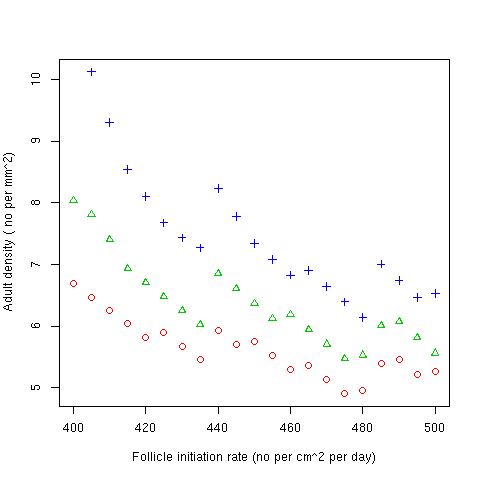
\includegraphics[width=0.9\textwidth]{slowfollinitratedens.png}
  \caption{Calculated values of adult follicle density at a range of values of the parameter $F_{r}$  from equations ~\ref{eqn:prim} to ~\ref{eqn:sd3} with values for the other 19  parameters fixed at the values given in Table~\ref{tab:base}. The three sets of points correspond to three values of the parameter $C_{b}$, red=.060, green=.062, blue=.064. The foetal growth rate in this graph has been changed from the base value of $B=.028$ to a slower value of $B=.024$.}
  \label{fig:slowfollinitratedens}
\end{figure}

%\end{document}

